\begin{figure}[h!]
  \centering
  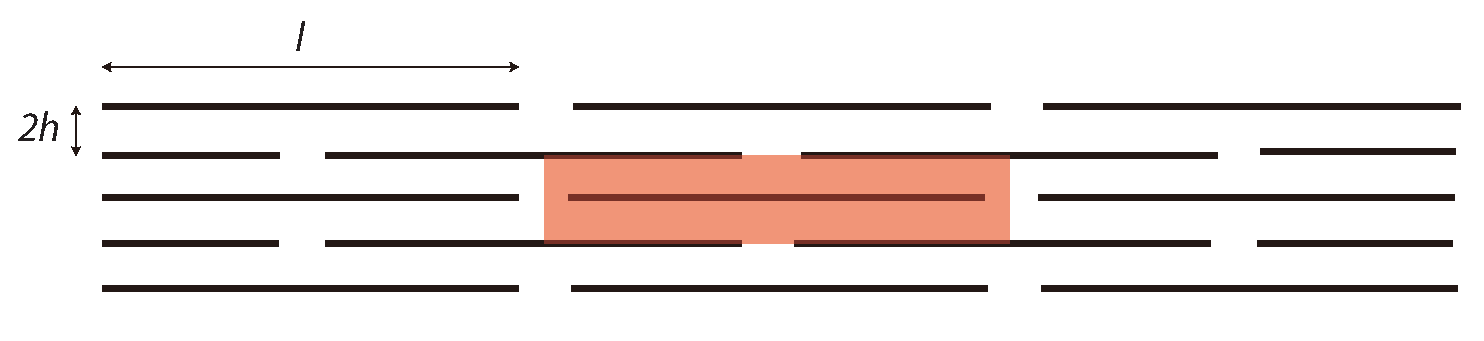
\includegraphics[width=5in]{paper4/FigS1.pdf}
  \caption{\textbf{Periodic cell used in the LB simulations.}}
  \label{figS1_AppC}
\end{figure}

Fig.~\ref{figS2_AppC} illustrates the dead-end filtration system, which is characterized by a reservoir (\textit{i.e.},
pressurized pot), allowing the filtration experiments to be performed with large volume (i.e.,
more than 3 L). The pressure taken from the wall was regulated with a pressure gauge from \textit{Ingersoll}. The membranes were placed in a stainless steel \textit{EDM Millipore holder}. 

\begin{figure}[h!]
  \centering
  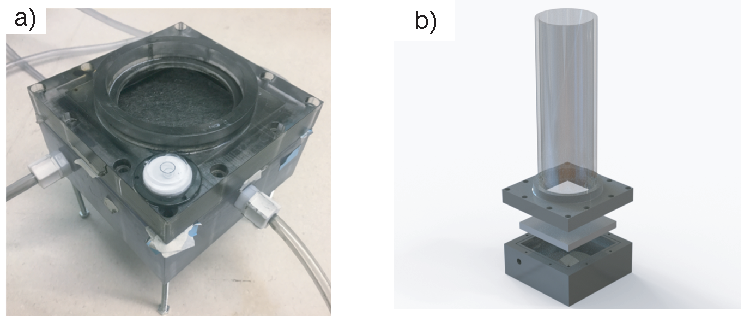
\includegraphics[width=4in]{paper4/FigS2.pdf}
  \caption{\textbf{Dead-end filtration set-up..}}
  \label{figS2_AppC}
\end{figure}


Table~\ref{tblS1_AppC} reports the oxygen and carbon footprints for the GOAL membranes. It is important to underline that the HI treatment is the most effective reduction technique among the ones tested and it allows achieving O/C ratio of 21\%. Regarding the UV irradiation, longer irradiation times lead to stronger reduction and the vacuum dictates more effective reduction compared to air. 

\begin{table}[t!]
 \begin{center}
 \caption{\textbf{XPS percentage peak area data for the six samples.} The standard deviation for the atomic ratio of each element is $\pm$1\%.}
  \label{tblS1_AppC}
  \begin{tabular}{*6c}
    Treatment & Time  & C-OH & C-C C=C & O-C-O & O/C \\
     &   & O-C-O &  & &  \\
    \hline
    Untreated &0 &68.56& 27.93 &3.51 &0.71 \\
    UV vacuum &20&57.27& 37.16& 5.57 &0.58\\
             & 60& 34.12& 57.81& 8.07& 0.52\\
             &360& 26.73& 61.91& 11.36 &0.46\\
             &720& 21.75 &70.62& 8.03& 0.39\\
             &1440& 13.87& 73.48& 12.65 &0.35\\
    UV air   &60 &37.79 &51.5& 10.67 &0.65\\
            &360& 38.12 &51.05& 10.83 &0.56\\
            &1440& 19.28& 66.21& 14.51& 0.46\\
    HI      & 1   &11.69 &76.46 &11.85 &0.21\\
    \hline
  \end{tabular}
 \end{center}
\end{table}


\begin{figure}[h!]
  \centering
  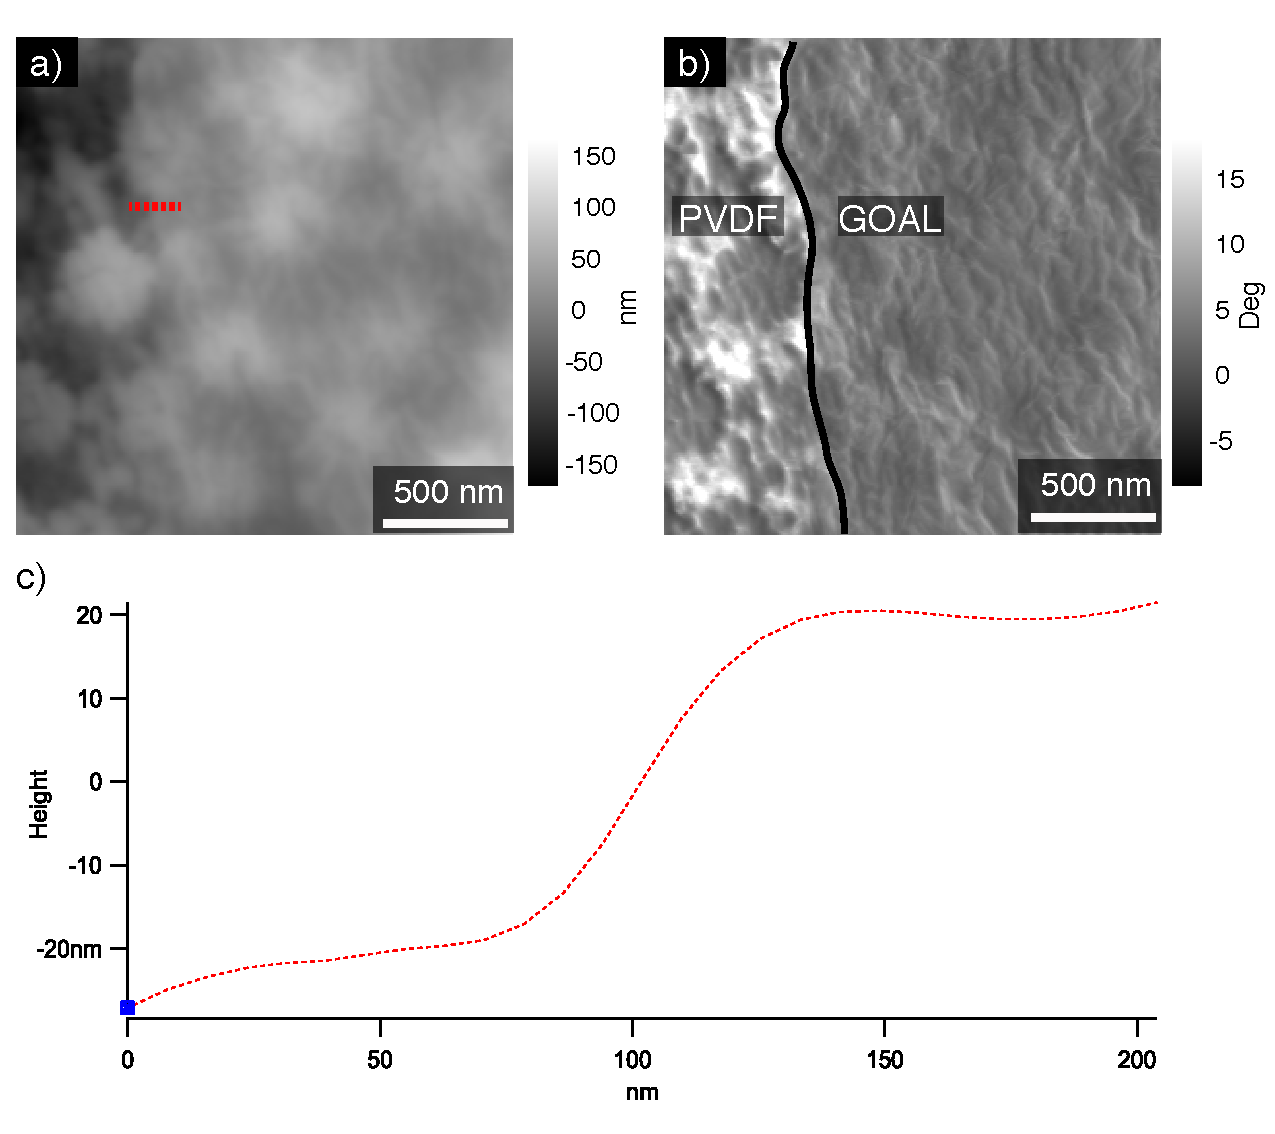
\includegraphics[width=5in]{paper4/FigS3.pdf}
  \caption{\textbf{AFM analysis of the GOAL surface.} \textbf{(a)} Topography, \textbf{(b)} phase image, \textbf{(c)} section line (in red)
acquired at the boundary between the GOAL and the bare PVDF. } 
  \label{figS3_AppC}
\end{figure}

AFM analysis of the GOAL surface at the boundary of the bare PVDF is displayed in Fig.~\ref{figS3_AppC}. Fig.~\ref{figS3_AppC}a represents the topography of the GOAL surface obtained and the dashed line section indicates a $<50$ nm topography variation (Fig.~\ref{figS3_AppC}c) at the interface between GO and PVDF, corroborating the SEM observations and mass analysis calculations on the thickness of the GO layer. The distinction between the two domains (GO and PVDF) is also visible in the phase image (Fig.~\ref{figS3_AppC}b) highlighting the different chemistry of the two materials. Fig.~\ref{figS4_AppC}a displays the evolution of the C1s spectrum with UV irradiation time in air. As explained in the main text, longer irradiation time leads to a more efficient graphitization of the GOAL. The intensity of the single (C-C) and double carbon (C=C) bond binding increases from 28\% to 51\%. This is also confirmed by the oxygen to carbon mass ratio (\textit{i.e.}, O/C) which decreases from 72\% to 56\% for untreated GOAL and the UV-GOAL irradiated for 360 min in air, respectively. Fig.~\ref{figS4_AppC}b represents the evolution of the XRD signal of GOAL with different UV irradiation times. We observed that the decrease in the number of functional groups with an increase in the exposure time leads to a shift of the peak of circa 1 {\AA}. However, as explained in the main text, the air treatment leads to a nosier XRD signal. 

\begin{figure}[h!]
  \centering
  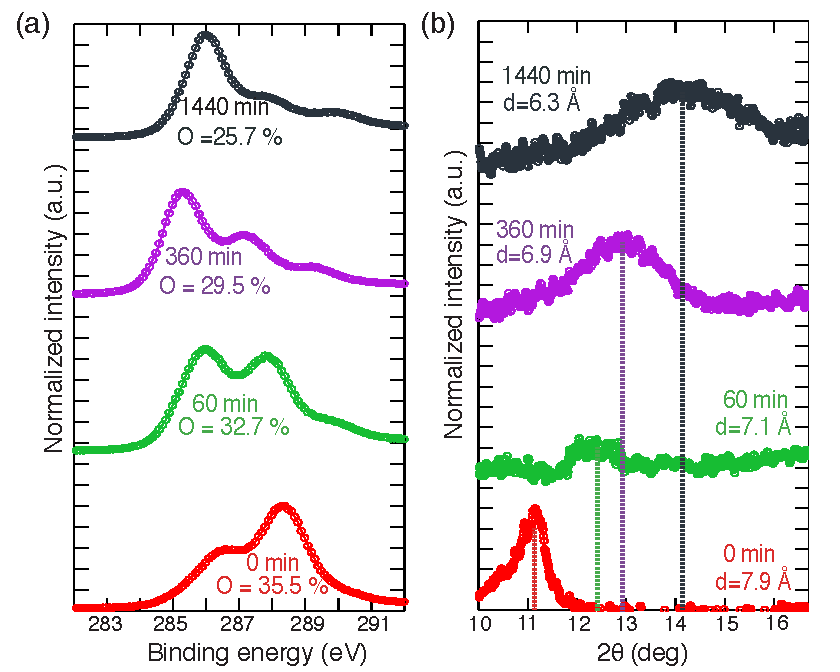
\includegraphics[width=4in]{paper4/FigS4.pdf}
  \caption{\textbf{GOAL oxygen content and interlayer spacing via UV reduction in air.} \textbf{(a)} XPS and \textbf{(b)} XRD spectra evolution for the UV irradiated GOAL membranes in air.} 
  \label{figS4_AppC}
\end{figure}

Fig.~\ref{figS5_AppC} represents the XPS and XRD spectra for HI-GOAL. We did not succeed in reducing the GO on Al\textsubscript{2}O\textsubscript{3} with HI and for this reason, we used PVDF as the substrate. As explained in the main text, the PVDF exhibits peaks in the same region of GO. However, in Fig.~\ref{figS5_AppC}a it is possible to notice the appearance of a peak centered at circa 16\textdegree. This peak, which was not as strong in the bare PVDF, can be related to the presence of the HI-GOAL and corresponds to a spacing of 5.5 {\AA}.

\begin{figure}[h!]
  \centering
  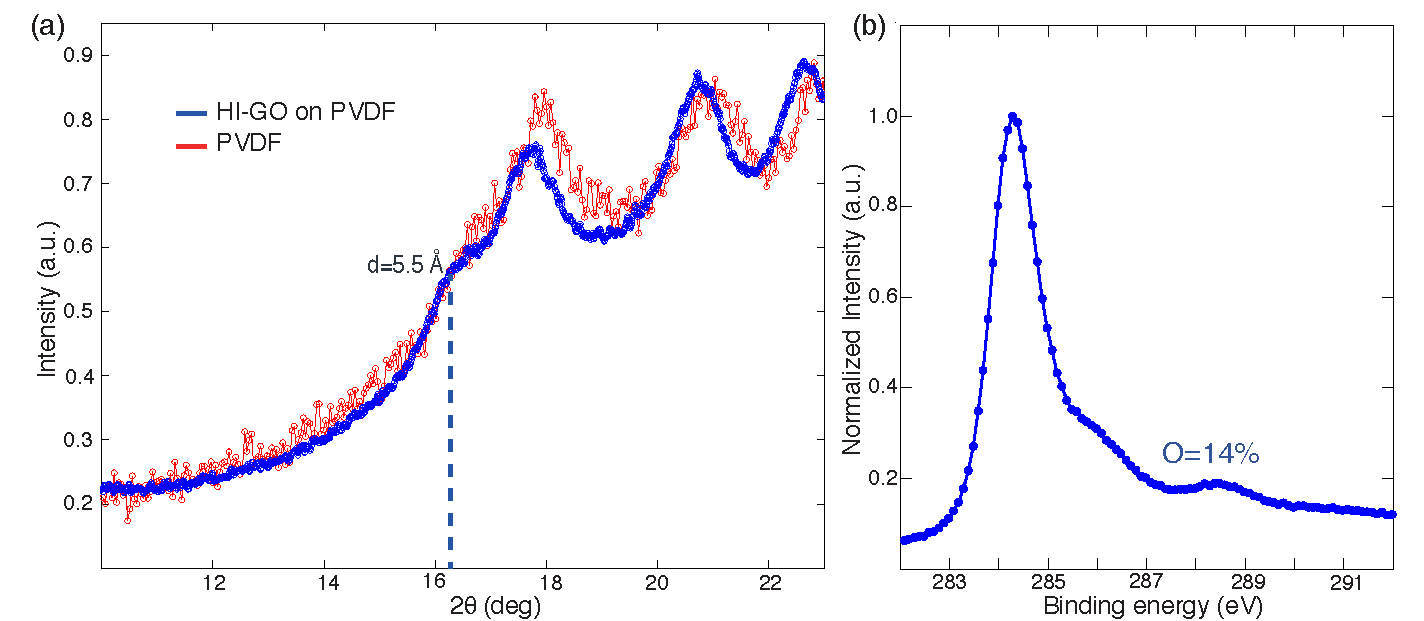
\includegraphics[width=6in]{paper4/FigS5.pdf}
  \caption{\textbf{ GOAL oxygen content and interlayer spacing via HI treatment.} \textbf{(a)} XRD and \textbf{(b)} XPS  spectrum for the GOAL treated with HI. } 
  \label{figS5_AppC}
\end{figure}

Fig.~\ref{figS6_AppC} represents the effect of the sonication treatment on the GO flake size. In particular,
with 23 min of bath sonication, the flake size varies from $52.2\pm18.9$ $\mu$m\textsuperscript{2} to $1.3\pm0.4$ $\mu$m\textsuperscript{2}.

\begin{figure}[h!]
  \centering
  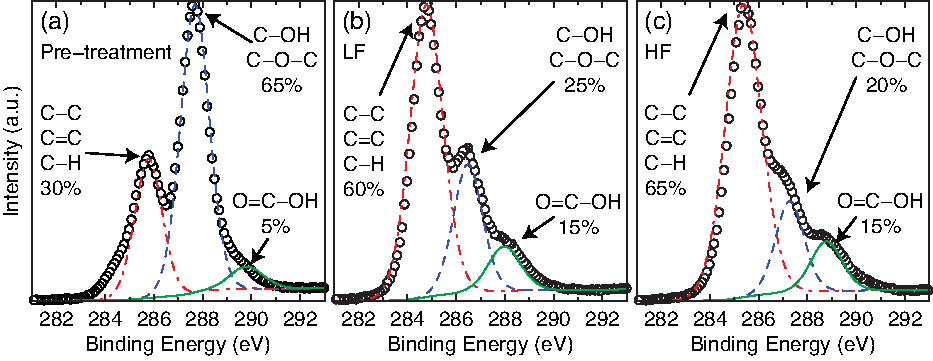
\includegraphics[width=6in]{paper4/FigS6.pdf}
  \caption{\textbf{SEM analysis of the sonication treatment.}  GO flakes size \textbf{(a)} before and \textbf{(b)} after ultrasonic irradiation.} 
  \label{figS6_AppC}
\end{figure}

Fig.~\ref{figS7_AppC} represents the independence between the variation of the dimensions of the GOAL architecture. Fig.~\ref{figS7_AppC}a displays the variation of the GO flake size versus the UV treatment time in vacuum. Although the UV treatment is responsible for the changing of the GOAL chemistry (\textit{i.e.}, the GOAL spacing), it is possible to notice that even 360 min of UV irradiation does not lead to a significant variation of the GO flake size. At the same time, the bath sonication treatment, responsible for the changing of the GO flake size, does not significantly change the chemical composition of the GOAL (Fig.~\ref{figS7_AppC}b). Moreover, the sonication does not change the spacing between the GO laminates as highlighted in the XRD spectra in Fig.~\ref{figS7_AppC}c. It is important to note that the sonication does not increase the GO defect density, which could lead to larger water permeability results. This is confirmed by three Raman intensity maps (4.096 acquisition points/spectra for an 80 x 80 $\mu$m\textsubscript{2} image with acquisition time 0.05 s/spectra) acquired for the sonicated and not-sonicated GO samples. The average D/G area ratio (A\textsubscript{D}/A\textsubscript{G}) for the three
images was evaluated to be $1.36\pm0.08$ and $1.38\pm0.05$ for the non-sonicated and the sonicated sample, respectively. 

\begin{figure}[h!]
  \centering
  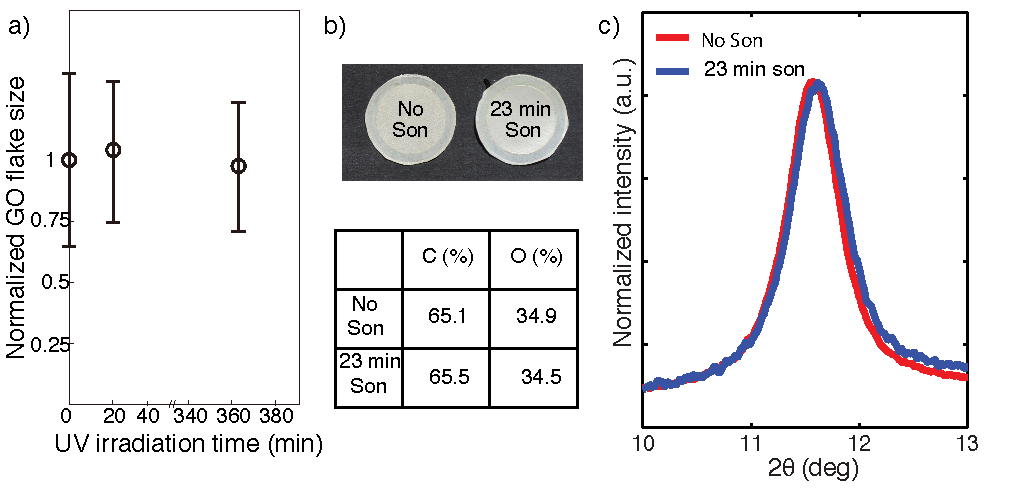
\includegraphics[width=5.5in]{paper4/FigS7.pdf}
  \caption{\textbf{Absence of interdependency between the tuning of flake size and oxygen content.} \textbf{(a)} Variation of the GO flake size with UV irradiation in vacuum. and \textbf{(b)} Photo of GOAL obtained with sonicated and not-sonicated GO solution and their atomic composition. \textbf{(c)} XRD spectra for GOAL obtained via GO sonicated for 23 min and notsonicated.} 
  \label{figS7_AppC}
\end{figure}

Fig.~\ref{figS8_AppC} represents the water permeation through a 0-GOAL membrane versus time. The initial permeability is characterized by higher values compared to the permeability at steady state conditions, which are reached after circa 700 min of filtration. In particular, during the membrane compaction stage, the permeability reduces by circa three-fold. The Darcy behavior of the membrane can also be observed with a pressure decrease from 3 to 1.2 bar, which leads to a reduction of permeability of almost a factor of three. The membrane permeability is also influenced by the GO thickness. Table~\ref{tblS2_AppC} reports permeability results for different amount of GO used for fabricating the membrane, which leads to different thickness.

\begin{figure}[h!]
  \centering
  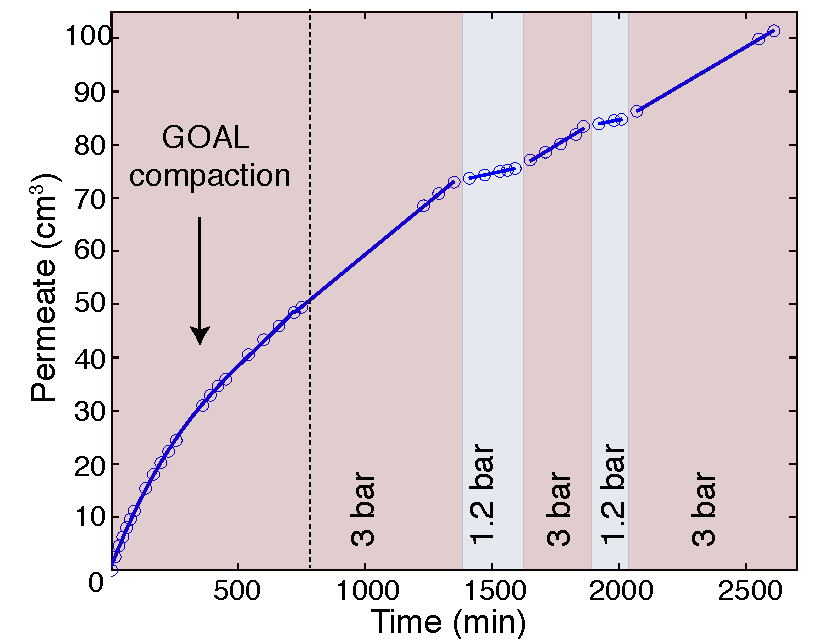
\includegraphics[width=4in]{paper4/FigS8.pdf}
  \caption{\textbf{Water permeation through 0-GOAL versus time.}} 
  \label{figS8_AppC}
\end{figure}


\begin{table}[t!]
 \begin{center}
 \caption{\textbf{Effect of the GO load (thickness) on the membrane permeability.}}
  \label{tblS2_AppC}
  \begin{tabular}{*2c}
    GO Amount & Permeability (LMH-bar)\\
    \hline
    1x & 2.18\\
    3x & 0.92\\
    4x & 0.65\\
    \hline
  \end{tabular}
 \end{center}
\end{table}

Fig.~\ref{figS9_AppC}, the GOAL structure was characterized via Raman spectroscopy and display a D-band (A\textsubscript{1g }symmetry) at $\approx1350$ cm\textsuperscript{-1} representative of defects/disorder in the basal plane and a
G-band (E\textsubscript{2g} symmetry) at $\approx1590$ cm\textsuperscript{-1}corresponding to the in-plane sp\textsuperscript{2} bond stretching, thus proportional to the extension of the graphitic domains. The longer exposure to UV irradiation leads to a smaller D/G peak intensity ratio (I\textsubscript{D}/I\textsubscript{G}). In particular, the I\textsubscript{D}/I\textsubscript{G} is equal to 0.95 and 0.90 for 15 min and 720 min UV irradiation, respectively, confirming the restoring of the graphitic domains via the reduction of GOAL. 
\begin{figure}[h!]
  \centering
  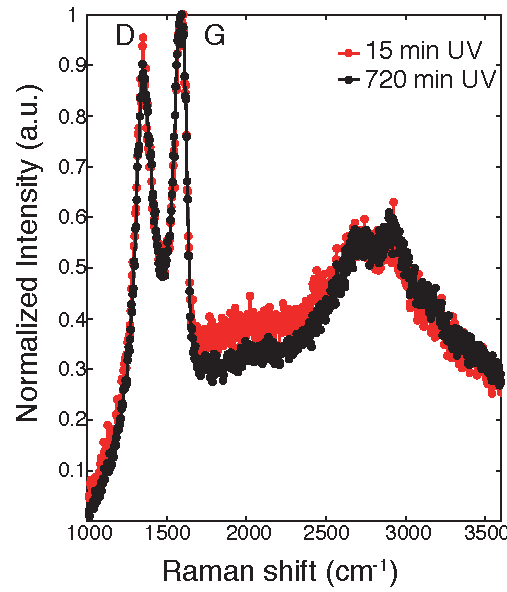
\includegraphics[width=3in]{paper4/FigS9.pdf}
  \caption{\textbf{ Raman D- and G-bands for 15minUV-GOAL and 720minUV-GOAL.}} 
  \label{figS9_AppC}
\end{figure}

Fig.~\ref{figS10_AppC} represents XRD spectra for reduced (UV-GOAL) and not reduced GOAL in a dry and hydrated state. As one can see, the hydration leads to smaller $2\theta$, which corresponds to a larger spacing ($2h$). In particular, when hydrated the spacing increased from 7.8 to 10.1 {\AA} and
from 8.1 to 10.5 {\AA} for UV-GOAL and GOAL, respectively. It is important to note that hydration affects the spacing to a similar degree (20-25\% increase) for both the oxidized and reduced GOAL in accordance with previously reported data.\cite{talyzin2014structure}

\begin{figure}[h!]
  \centering
  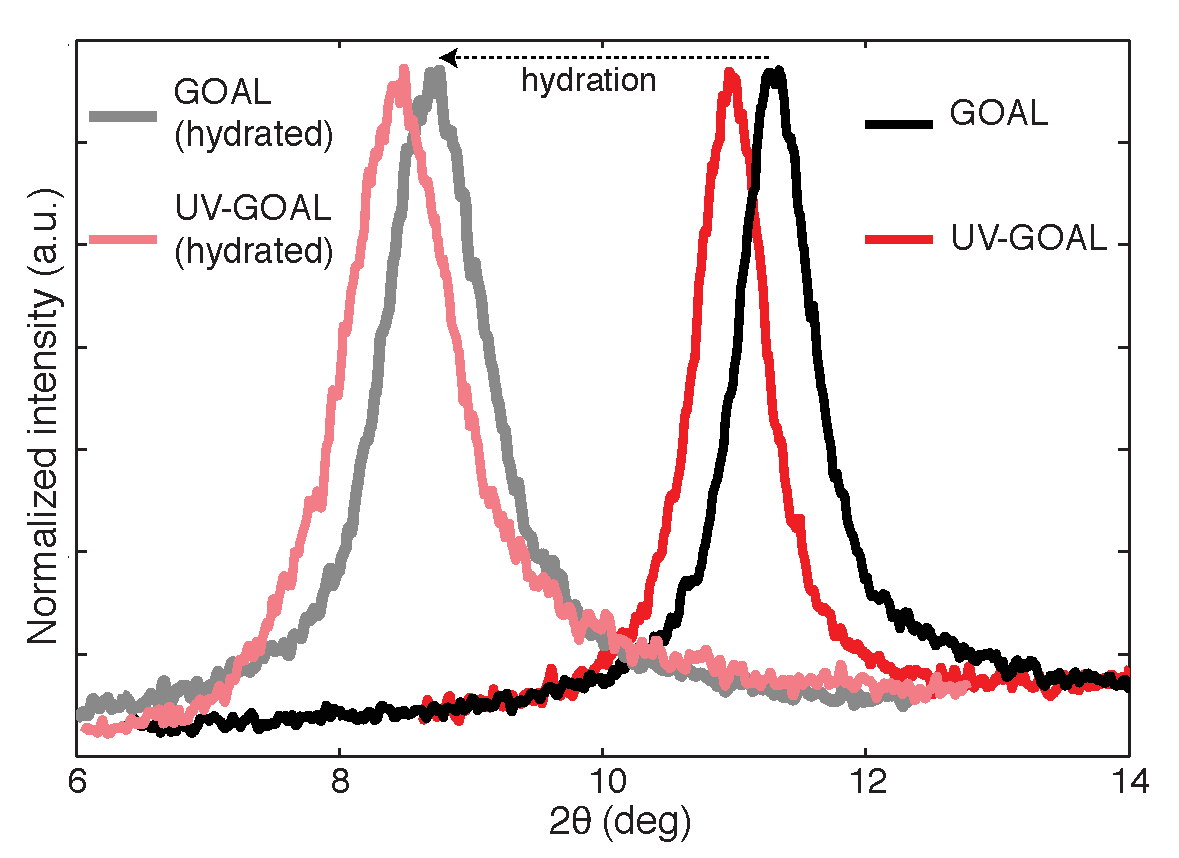
\includegraphics[width=4in]{paper4/FigS10.pdf}
  \caption{\textbf{XRD spectra for hydrated GOAL and UV-GOAL.}} 
  \label{figS10_AppC}
\end{figure}

Table~\ref{tblS3_AppC} and Table~\ref{tblS4_AppC} represent the variation in the permeability ($\Delta k$) due to the chemical reduction and sonication, respectively. The tables also report the normalized variations ($\Delta k_{2h}$ and $\Delta k_{l}$) for each scenario. As explained in the main text, the larger values of $\Delta 2h$ highlight the importance of the nanochannels interlayer spacing in dictating the permeability, compared to the length of the nanochannels. 

\begin{table}
 \begin{center}
 \caption{\textbf{Effect of the GO nanochannels interlayer spacing ($2h$) on the permeability.}}
  \label{tblS3_AppC}
  \begin{tabular}{*7c}
     &15-GOAL&360-GOAL&HI-GOAL&15-GOAL-son&360-GOAL-son&HI-GOAL-son\\
    \hline
    $\Delta k$ (\%)  & 56 &74& 91 &43 &66 &86\\
    $\Delta k_{2h}$& 6.35& 5.3 &3.0& 5.0& 4.7& 2.8 \\
    \hline
  \end{tabular}
 \end{center}
\end{table}


\begin{table}
 \begin{center}
 \caption{\textbf{Effect of the GO nanochannels interlayer spacing ($l$) on the permeability.}}
  \label{tblS4_AppC}
  \begin{tabular}{*7c}
    {}&0-GOAL-son&15-GOAL-son&360-GOAL-son&HI-GOAL-son\\
    \hline
    $\Delta k$ (\%) & 19 &53& 60 & 110\\
    $\Delta k_{l}$& 0.02& 0.08 &0.09& 0.15 \\
    \hline
  \end{tabular}
 \end{center}
\end{table}

